\begin{figure}
	\begin{center}
		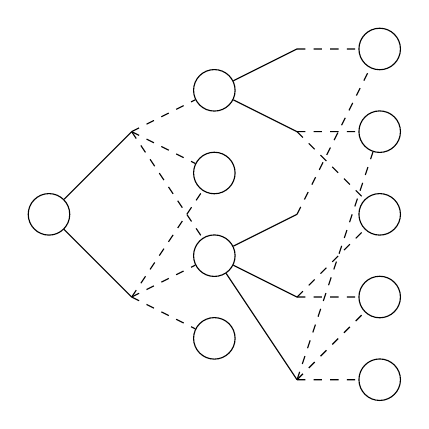
\begin{tikzpicture}[
			wide/.style={line width=4pt}, every node/.style={circle,draw,minimum size=15}, scale=.35]

			\node (root) at (-6,0) {};

			\coordinate (branch1) at (-3, 3) {};
			\coordinate (branch2) at (-3, -3) {};

			\node  (s1) at (0, 4.5) {};
			\node  (s2) at (0, 1.5) {};
			\node  (s3) at (0, -1.5) {};
			\node  (s4) at (0, -4.5) {};

			\coordinate (branch3) at (3, 6) {};
			\coordinate (branch4) at (3, 3) {};
			\coordinate (branch5) at (3, 0) {};
			\coordinate (branch6) at (3, -3) {};
			\coordinate (branch7) at (3,-6) {};

			\node  (s5) at (6, 6) {};
			\node  (s6) at (6, 3) {};
			\node  (s7) at (6, 0) {};
			\node  (s8) at (6, -3) {};
			\node  (s9) at (6,-6) {};

			\draw (root) -- (branch1);
			\draw (root) -- (branch2);

			\draw[dashed] (branch1) -- (s1);
			\draw[dashed]  (branch1) -- (s2);
			\draw[dashed]  (branch1) -- (s3);

			\draw[dashed] (branch2) -- (s2);
			\draw[dashed]  (branch2) -- (s3);
			\draw[dashed]  (branch2) -- (s4);

			\draw (s1) -- (branch3);
			\draw (s1) -- (branch4);

			\draw (s3) -- (branch5);
			\draw (s3) -- (branch6);
			\draw (s3) -- (branch7);

			\draw[dashed] (branch3) -- (s5);

			\draw[dashed] (branch4) -- (s6);
			\draw[dashed]  (branch4) -- (s7);

			\draw[dashed] (branch5) -- (s5);

			\draw[dashed] (branch6) -- (s7);
			\draw[dashed] (branch6) -- (s8);


			\draw[dashed] (branch7) -- (s9);
			\draw[dashed]  (branch7) -- (s6);
			\draw[dashed]  (branch7) -- (s8);

		\end{tikzpicture}

		\caption{
			An example of a general Markov Search Process (MSP), with the starting state on the left and time moving from left to right.
			States are given by nodes in the graph.
			Solid lines represent available actions, while dotted lines represent possible randomized state transitions given the chosen action.
		}
	\end{center}
\end{figure}
